
\chapter{SYSTEM IMPLEMENTATION }
\thispagestyle{empty}
\\
\section{introduction}
\hspace{.2cm} The data analysis done in the previous chapter indicates that the automation of the 
processes of carrying out, monitoring and recording business transactions of Avenue Event Planners can lead to reduction in cost of doing business, improved data 
management and quick decision-making process. Details of reliable and timely 
information about the different events scheduled. 
The database used to store the information was separated from the user interface and 
business logic. MongoDB was used to implement the database and a combination of HTML ,CSS
and JavaScript were used for the implementation of the interfaces.NodeJS was used for implementing the backend 
logic . 
\section{Implementation }
The table below shows the different activities and deliverables of the online Event Management System. 
\begin{table}[]
	\centering
	\caption{\textbf{System implementation plan }}
	\label{table }
	\begin{tabular}{|p{4.5cm}|p{4.5cm}|p{4.5cm}|}
		\hline
		Activity  & Tools Used &	Deliverables \\
		
		\hline
		Database Implementation&
		MongoDB 6.0 ,MongoDB Atlas
		& 
		Fully operational and working Database.
		
		\\
		\hline
		Implementation of Interfaces &
		HTML5, CSS ,Bootstrap
		
		&
		User friendly interfaces  
		\\
		\hline
		Implementation of business Logic &
		JavaScript, NodeJS 18
		&
		System code, 
		\\
		\hline
	\end{tabular}
\end{table}
\newpage
\begin{table}
	\centering
	
	\label{table }
	\begin{tabular}{|p{4.5cm}|p{4.5cm}|p{4.5cm}|}
		\hline
		System Testing&
		NodeJS 18, MongoDB, HTML5, CSS , Apache 
		2.0.22
		&	
		System reviewed, System 
		security tested. 
		\\
		\hline
		
	\end{tabular}
\end{table}
\section{Database Implementation  }
\hspace{.2cm} 
MongoDB DBMS and MongoDB Atlas interface were used to create the database and all 
tables. The 
figure below shows a screen shot of the database and all the collections in the database. 
\begin{figure}[h]
	\centering
	\includegraphics[scale=0.3]{DbImplementation.png}
	\caption{Database with all the Collections}
	\label{Database with all the Collections}
\end{figure}
\begin{figure}[h]
	\centering
	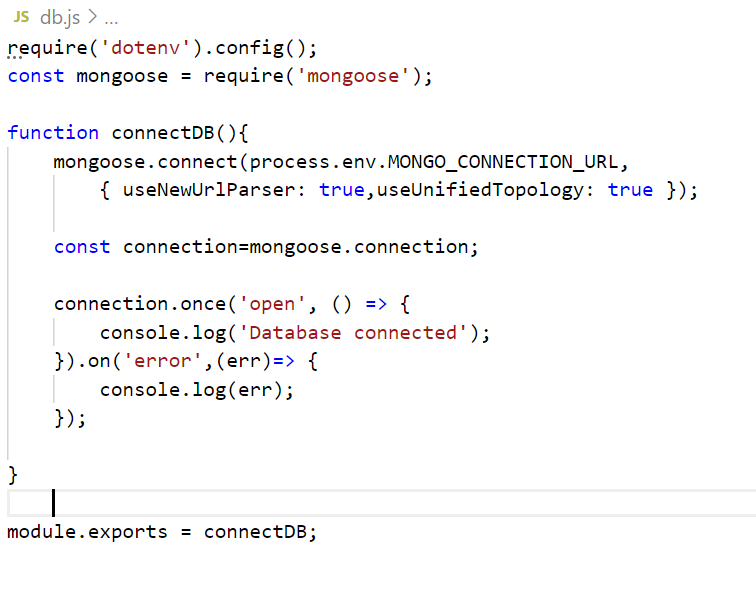
\includegraphics[scale=0.4]{DBconnection.png}
	\caption{Database Connection}
	\label{Database Connection}
\end{figure}
\section{ Implementation of User Interfaces   }


\hspace{.2cm} 
The UI of the website is developed using html5, css and javascript, Bootstrap framework is also used to make our website more responsive.

\begin{figure}[h]
	\centering
	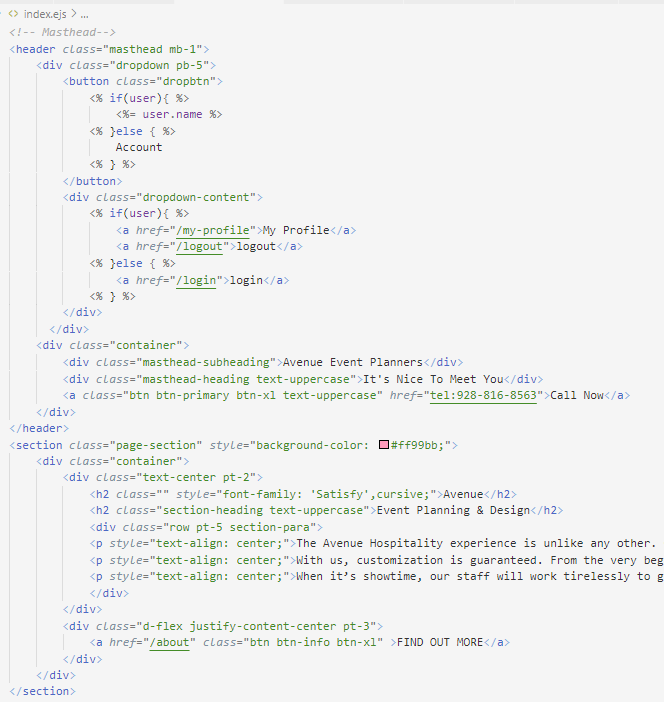
\includegraphics[scale=0.5]{homecode1.png}
	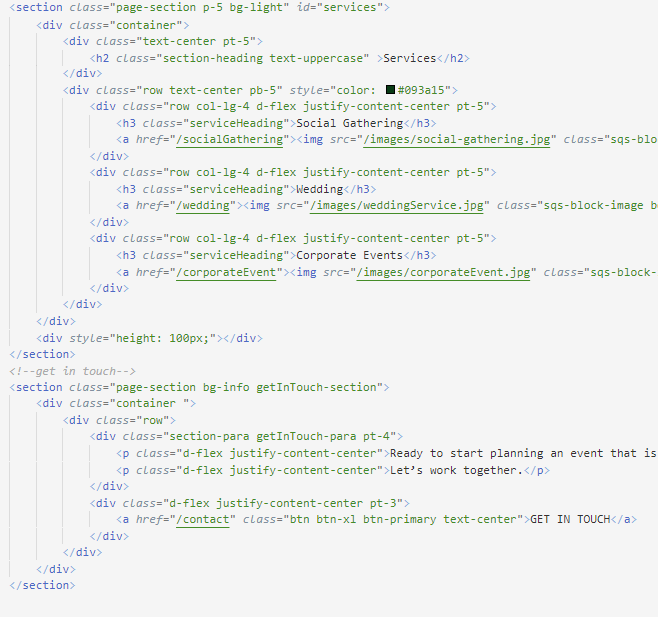
\includegraphics[scale=0.5]{homecode2.png}
	\caption{Implementation of home page}
	\label{Implementation of home page}
\end{figure}

\begin{figure}[H]
	\centering
	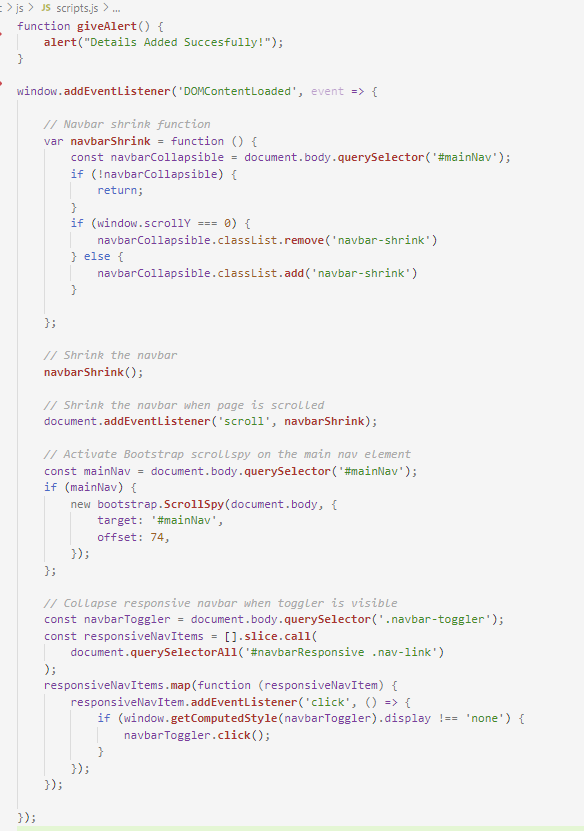
\includegraphics[scale=0.5]{scripts.png}
	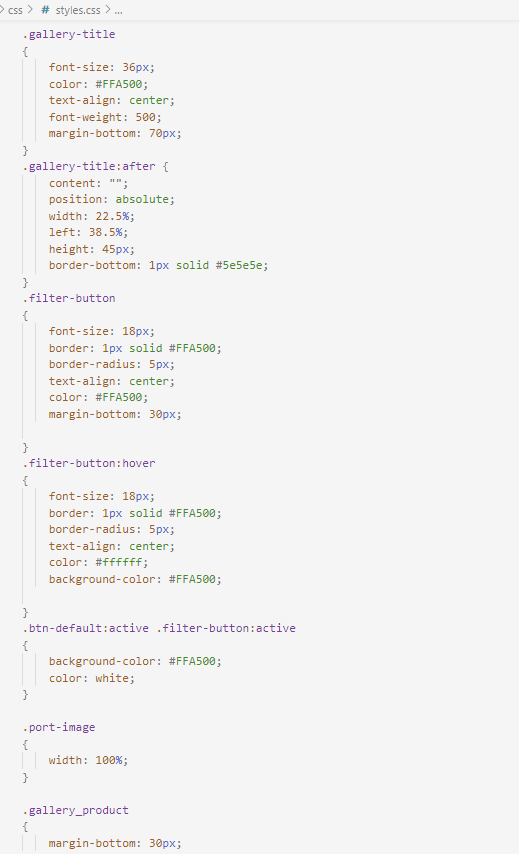
\includegraphics[scale=0.5]{styles.png}
	\caption{JavaScripts and CSS Implementation}
	\label{JavaScripts and CSS Implementation}
\end{figure}

\section{ Implementation of Business Logic(BackEnd)  }

\hspace{.2cm} 
The backend handle everything that doesn't involve providing a user interface. This can include writing APIs, building libraries, and utilities.Nodejs is used as a language for the backend. Express.js which is a framework for nodejs is used building the website and APIs.
\begin{figure}[H]
	\centering
	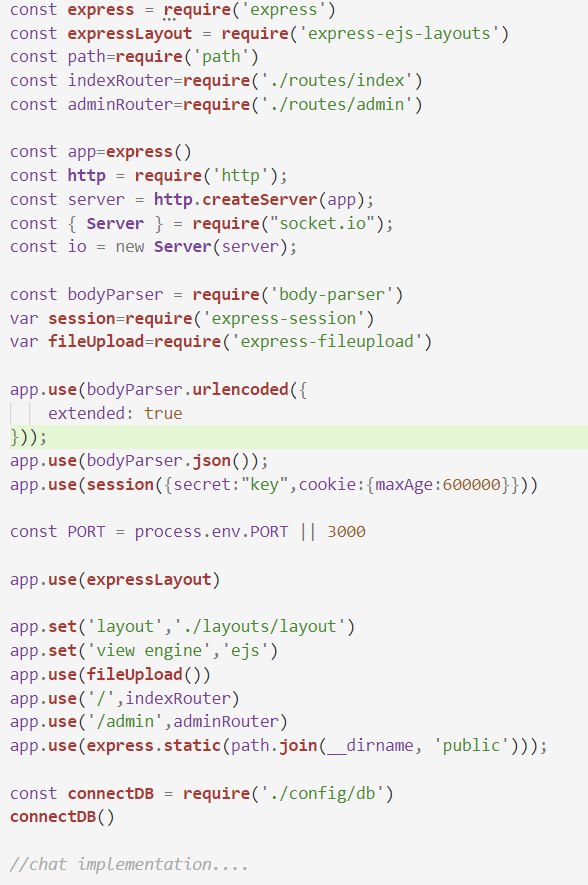
\includegraphics[scale=0.5]{server1.png}
	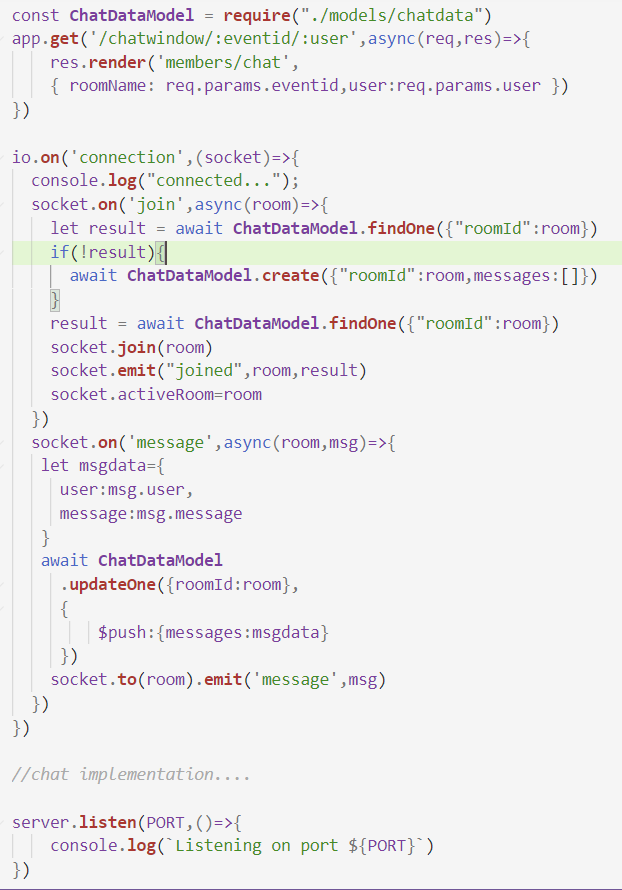
\includegraphics[scale=0.5]{server2.png}
	\caption{BackEnd Server.js }
	\label{BackEnd Server.js}
\end{figure}

\begin{figure}[H]
	\centering
	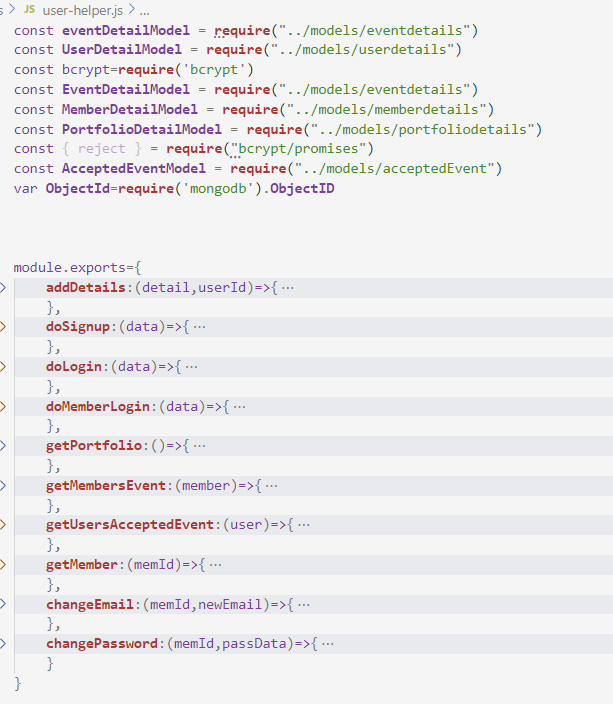
\includegraphics[scale=0.5]{helperfunctions1.png}
	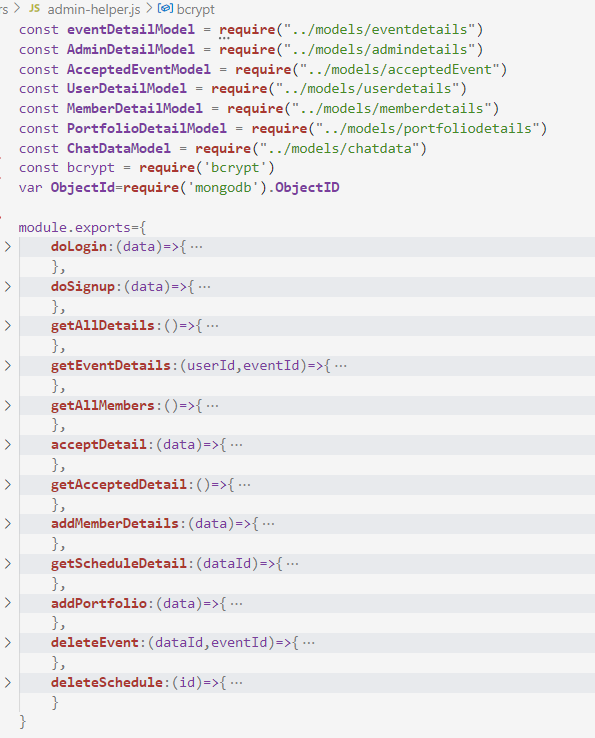
\includegraphics[scale=0.5]{helperfunctions2.png}
	\caption{Backend Helper Functions }
	\label{Backend Helper Functions}
\end{figure}
\section{ Implementation of Mailing Service   }

\hspace{.2cm} 
Mail service is also included in the Online Event Management System. SendInBlue mail service is used to sent mail to the client, members and the admin. It's one of the best tools for trigger-based and transactional emails. Its automation workflow designer allows you to build campaigns triggered by clicks, opens and even webpage visits.

\begin{figure}[h]
	\centering
	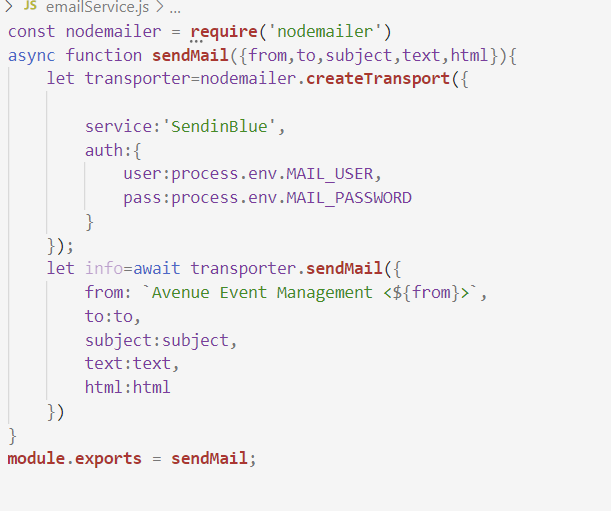
\includegraphics[scale=0.5]{mailservice.png}
	\caption{ Mailing service.js }
	\label{ Mailing service.js }
\end{figure}




 


\\\\



\\\\
